\subsubsection{Szczegóły budowania zbioru helpful}
Główna funkcja tej heurystyki działa podobnie do algorytmu Kruskala do wyliczania
najmniejszego drzewa rozpinającego \cite{algorithms222}.
Startuje od pustego zbioru (o wartości helpfulness równej $0$) i buduje go za pomocą wierzchołków z jednej strony granicy.
W każdym kroku wybiera wierzchołek z wartością helpfulness z pewnego przedziału, przenosi go do zbioru
(helpfulness zbioru zwiększa się wtedy o helpfulness wierzchołka), następnie zwiększa wartość helpfulness wierzchołków,
które są w tej samej partycji i są sąsiednie do przeniesionego wierzchołka,
Te wierzchołki zyskują jedną krawędź zewnętrzną
kosztem jednej krawędzi wewnętrznej, w związku z powyższym ich wartość helpfulness rośnie o $2$.
\begin{figure}[h]
    \centering
    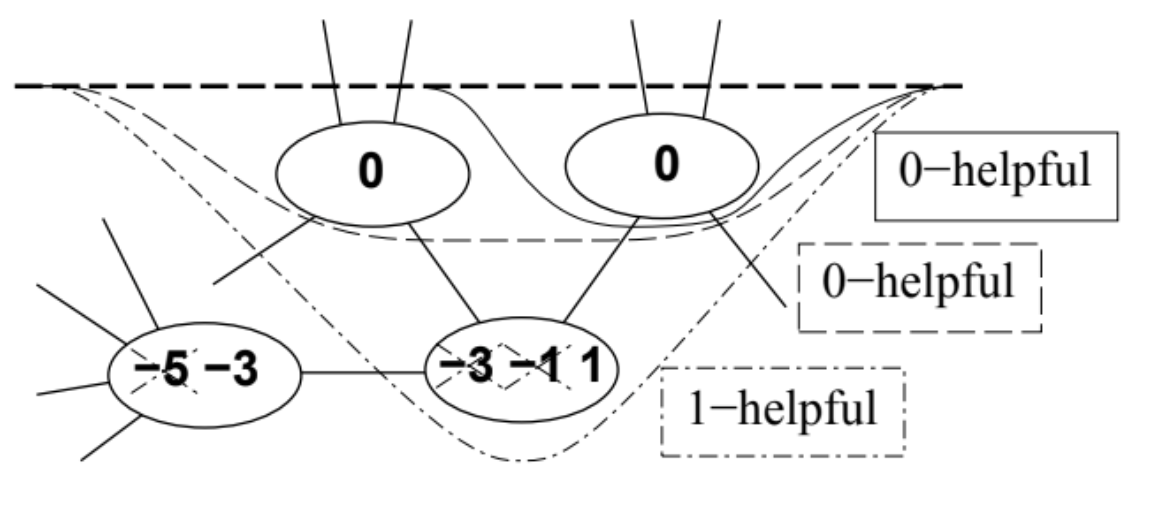
\includegraphics[width=0.6\linewidth]{images/changing_helpful_values}
    \caption{Zmiana wartości helpfulness dla sąsiadów.
    Źródło: \cite{article}.}
    \label{im:helpfulness_neighbours}
\end{figure}

Branie pod uwagę tylko wierzchołków z jednej strony granicy pozwala na budowanie zbioru z dwóch stron podziału jednocześnie.
Jeśli znaleziony zbiór wierzchołków jest przemieszczany między partycjami, to wartości helpfulness dla wierzchołków
docelowej partycji muszą również zostać zaktualizowane.
Podczas budowania zbioru jego wielkość zwiększa się w każdym kroku.
Zbiór helpful przestaje być budowany w następujących przypadkach:
\begin{itemize}
    \item wartość helpfulness dla zbioru osiągnie wartość limitu,
    \item {brane są pod uwagę tylko wierzchołki o pewnej wartości helpfulness, a te się skończą,}
    \item wielkość zbioru osiągnie wartość limitu.
\end{itemize}
Ważną obserwacją jest fakt, że jeśli brane pod uwagę są jedynie wierzchołki z wartością helpfulness $\geq$ $0$,
to helpfulness zbioru albo zachowuje tę samą wartość, albo rośnie, ale nigdy nie maleje.
Podobieństwo tego algorytmu do algorytmu BFS objawia się w sposobie, w jakim wierzchołki przypisywane są do zbioru.
Wierzchołek może zostać wybrany, jeśli jego wartość helpfulness jest większa od ustalonej wartości.
To następuje albo jeśli wierzchołek ma od początku odpowiednią wartość helpfulness, albo jeśli urośnie ona do odpowiedniej
wartości podczas budowania zbioru (poprzez dodanie do zbioru jego sąsiadów).

\newpage
\begin{figure}[h]
\begin{subfigure}{.32\textwidth}
    \centering
    \fbox{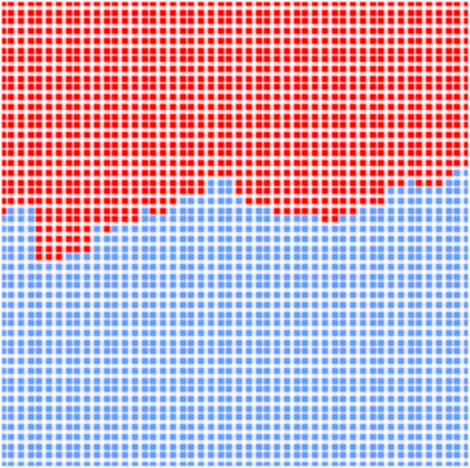
\includegraphics[width=0.7\textwidth]{images/building-helpfulsets/3}}
    \caption[short]{podział}
\end{subfigure}
\begin{subfigure}{.32\textwidth}
    \centering
    \fbox{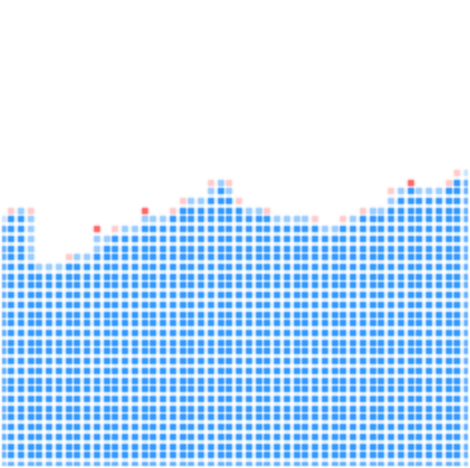
\includegraphics[width=0.7\textwidth]{images/building-helpfulsets/4}}
    \caption[short]{wartości helpfulness wierzchołków}
\end{subfigure}
\begin{subfigure}{.32\textwidth}
    \centering
    \fbox{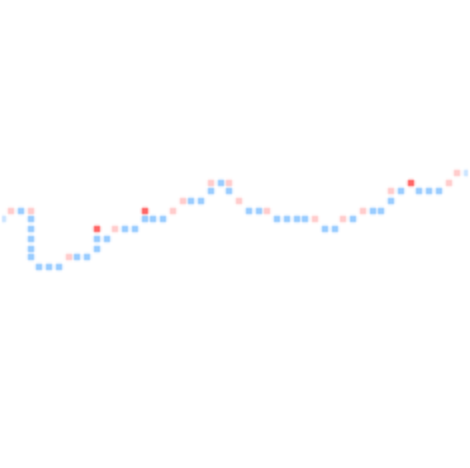
\includegraphics[width=0.7\textwidth]{images/building-helpfulsets/5}}
    \caption[short]{wierzchołki do budowania zbioru helpful}
\end{subfigure}
\caption{Obrazki przedstawiają jak wygląda zbiór wierzchołków, na bazie którego budowany jest zbiór helpful.
Obrazek (a) przedstawia partycjonowanie. Zbiór helpful będzie budowany na niebieskiej partycji.
Obrazek (b) przedstawia wszystkie wierzchołki zbioru (a), gdzie kolor oznacza wartość helpful. Skala rozpoczyna się od
koloru ciemnoniebieskiego dla wierzchołków z wartością helpfulness wynoszącą $-4$ i przechodzi do czerwonego dla wierzchołków z
wartością helpfulness $4$. Widoczna jest większa wartość helpfulness dla wierzchołków przy granicy. Obrazek (c)
przedstawia wierzchołki, które brane są pod uwagę przez algorytm. Są one filtrowanie na etapie budowania zbioru,
tak by zawsze wybierane były wierzchołki znajdujące się na granicy.}
\label{im:building_helpfulsets}
\end{figure}

Dodatkową modyfikacją, którą wprowadziłem, było filtrowanie wierzchołków, tak by algorytm wybierał wierzchołek z największą
wartością helpfulness tylko spośród wierzchołków granicznych.
Została ona zaimplementowana w związku z powstającymi obszarami rozproszonymi
(to negatywne zjawisko opisuje w późniejszych częściach pracy).
Chciałem aby istniała pewność, że wybierany wierzchołek jest zawsze wierzchołkiem granicznym.
Rysunek \ref{im:building_helpfulsets} przedstawia moje rozwiązanie.